% Use the following line _only_ if you're still using LaTeX 2.09.
%\documentstyle[icml2014,epsf,natbib]{article}
% If you rely on Latex2e packages, like most modern people use this:
\documentclass{article}

% use Times
\usepackage{times}
% For figures
\usepackage{graphicx} % more modern
%\usepackage{epsfig} % less modern
\usepackage{subfigure} 

% For citations
\usepackage{natbib}

% For algorithms
%\usepackage{algorithm}
%\usepackage{algorithmic}
%\usepackage{algorithmicx}

% As of 2011, we use the hyperref package to produce hyperlinks in the
% resulting PDF.  If this breaks your system, please commend out the
% following usepackage line and replace \usepackage{icml2014} with
% \usepackage[nohyperref]{icml2014} above.
\usepackage{hyperref}

% Packages hyperref and algorithmic misbehave sometimes.  We can fix
% this with the following command.
\newcommand{\theHalgorithm}{\arabic{algorithm}}

% Employ the following version of the ``usepackage'' statement for
% submitting the draft version of the paper for review.  This will set
% the note in the first column to ``Under review.  Do not distribute.''
\usepackage{format/icml2014} 
% Employ this version of the ``usepackage'' statement after the paper has
% been accepted, when creating the final version.  This will set the
% note in the first column to ``Proceedings of the...''
%\usepackage[accepted]{icml2014}

\usepackage{times}
\usepackage{hyperref}
\usepackage{url}
\usepackage{color}
\usepackage{preamble}
\definecolor{mydarkblue}{rgb}{0,0.08,0.45}
\hypersetup{ %
    pdftitle={},
    pdfauthor={},
    pdfsubject={},
    pdfkeywords={},
    pdfborder=0 0 0,
    pdfpagemode=UseNone,
    colorlinks=true,
    linkcolor=mydarkblue,
    citecolor=mydarkblue,
    filecolor=mydarkblue,
    urlcolor=mydarkblue,
    pdfview=FitH}
    
    
\usepackage{amsmath, amsfonts, bm, lipsum, capt-of}
\usepackage{natbib, xcolor, wrapfig, booktabs, multirow, caption}
\DeclareCaptionType{copyrightbox}
\usepackage{float}


%\renewcommand{\baselinestretch}{0.99}

\def\ie{i.e.\ }
\def\eg{e.g.\ }
\let\oldemptyset\emptyset
\let\emptyset\varnothing

%\author{
%James Robert Lloyd\\
%University of Cambridge\\
%Department of Engineering\\
%\texttt{jrl44@cam.ac.uk}
%\And
%David Duvenaud\\
%University of Cambridge \\
%Department of Engineering \\
%\texttt{dkd23@cam.ac.uk}
%\And
%Roger Grosse\\
%M.I.T.\\
%Brain and Cognitive Sciences \\
%\texttt{rgrosse@mit.edu}
%\And
%Joshua B. Tenenbaum\\
%M.I.T.\\
%Brain and Cognitive Sciences \\
%\texttt{jbt@mit.edu}
%\And
%Zoubin Ghahramani\\
%University of Cambridge \\
%Department of Engineering \\
%\texttt{zoubin@eng.cam.ac.uk}
%}

\newcommand{\fix}{\marginpar{FIX}}
\newcommand{\new}{\marginpar{NEW}}

\setlength{\marginparwidth}{0.6in}
%%%%%%%%%%%%%%%%%%%%%%%%%%%%%%%%%%%%%%%%%%%%%%%%%%%%%%%%%%
%%%% EDITING HELPER FUNCTIONS  %%%%%%%%%%%%%%%%%%%%%%%%%%%
%%%%%%%%%%%%%%%%%%%%%%%%%%%%%%%%%%%%%%%%%%%%%%%%%%%%%%%%%%

%% NA: needs attention (rough writing whose correctness needs to be verified)
%% TBD: instructions for how to fix a gap ("Describe the propagation by ...")
%% PROBLEM: bug or missing crucial bit 

%% use \fXXX versions of these macros to put additional explanation into a footnote.  
%% The idea is that we don't want to interrupt the flow of the paper or make it 
%% impossible to read because there are a bunch of comments.

%% NA's (and TBDs, those less crucially) should be written so 
%% that they flow with the text.

\definecolor{WowColor}{rgb}{.75,0,.75}
\definecolor{SubtleColor}{rgb}{0,0,.50}

% inline
\newcommand{\NA}[1]{\textcolor{SubtleColor}{ {\tiny \bf ($\star$)} #1}}
\newcommand{\LATER}[1]{\textcolor{SubtleColor}{ {\tiny \bf ($\dagger$)} #1}}
\newcommand{\TBD}[1]{\textcolor{SubtleColor}{ {\tiny \bf (!)} #1}}
\newcommand{\PROBLEM}[1]{\textcolor{WowColor}{ {\bf (!!)} {\bf #1}}}

% as margin notes

\newcounter{margincounter}
\newcommand{\displaycounter}{{\arabic{margincounter}}}
\newcommand{\incdisplaycounter}{{\stepcounter{margincounter}\arabic{margincounter}}}

\newcommand{\fTBD}[1]{\textcolor{SubtleColor}{$\,^{(\incdisplaycounter)}$}\marginpar{\tiny\textcolor{SubtleColor}{ {\tiny $(\displaycounter)$} #1}}}

\newcommand{\fPROBLEM}[1]{\textcolor{WowColor}{$\,^{((\incdisplaycounter))}$}\marginpar{\tiny\textcolor{WowColor}{ {\bf $\mathbf{((\displaycounter))}$} {\bf #1}}}}

\newcommand{\fLATER}[1]{\textcolor{SubtleColor}{$\,^{(\incdisplaycounter\dagger)}$}\marginpar{\tiny\textcolor{SubtleColor}{ {\tiny $(\displaycounter\dagger)$} #1}}}


%% For submission, make all render blank.
%\renewcommand{\LATER}[1]{}
%\renewcommand{\fLATER}[1]{}
%\renewcommand{\TBD}[1]{}
%\renewcommand{\fTBD}[1]{}
%\renewcommand{\PROBLEM}[1]{}
%\renewcommand{\fPROBLEM}[1]{}
%\renewcommand{\NA}[1]{#1}  % Note, NA's pass through!


% The \icmltitle you define below is probably too long as a header.
% Therefore, a short form for the running title is supplied here:
\icmltitlerunning{Automatic construction and natural-language summarization of additive nonparametric models}

\begin{document} 

\twocolumn[
\icmltitle{Automatic construction and natural-language summarization\\of additive nonparametric models}

% It is OKAY to include author information, even for blind
% submissions: the style file will automatically remove it for you
% unless you've provided the [accepted] option to the icml2014
% package.
\icmlauthor{Your Name}{email@yourdomain.edu}
\icmladdress{Your Fantastic Institute,
            314159 Pi St., Palo Alto, CA 94306 USA}
\icmlauthor{Your CoAuthor's Name}{email@coauthordomain.edu}
\icmladdress{Their Fantastic Institute,
            27182 Exp St., Toronto, ON M6H 2T1 CANADA}

% You may provide any keywords that you 
% find helpful for describing your paper; these are used to populate 
% the "keywords" metadata in the PDF but will not be shown in the document
\icmlkeywords{}

\vskip 0.3in
]

\begin{abstract} 
One of the broad aims of statistics is to produce an accurate and concise description of data.
Parametric techniques typically produces a concise description of data but can be inaccurate when there are deviations from the strong assumptions implied by parametric forms.
In contrast, nonparametric methods are typically capable of providing accurate descriptions of many data sets but at the expense of succinct descriptions.
To address this apparent antagonism we demonstrate that a recently introduced nonparametric model construction technique allows for the automatic natural-language description of a data set into natural-language while also constructing an accurate model.
We also extend the class of models that can be produced by this model construction method to include a wide variety of regression motifs.
\end{abstract} 

\allowdisplaybreaks

\section{Introduction}

Simple parametric regression models such as linear regression are usually easily interpretable, requiring only a table of regression coefficients and a few other parameters to describe the model.
In contrast, non-parametric models typically require graphical descriptions of their fit since any text description would be overly simplistic (\eg `a smooth function') and fitted parameters correspond only to very high level concepts such as bandwidths or typical lengthscales.

Several recently proposed methods search over a large class of structured nonparametric regression models \citep{DuvLloGroetal13, kronberger2013evolution, diosan2007evolving, bing2010gp}.
In \citep{DuvLloGroetal13}, it was noted that these models could be decomposed into sums of diverse components, and that the different components corresponded to interpretable features of the data.
In that work, components discovered on real datasets were interpreted post-hoc by the authors.

We extend this work by demonstrating that the compositional structure of the models searched over allows for the automatic natural-language description of patterns within a data set \ie the interpretable models are automatically interpreted!
We also expand and improve the components used in the model-construction process to improve the expressivity and interpretability of the models.
This allows for the procedure to fit and describe many well established modelling motifs including, linear regression, Fourier analysis, sparse spectrum \gp{}s (cite), changepoints (cite), heteroscedasiticty (cite), trend-cyclical-irregular (cite) and nonparametric additive / MKL (cite).

This manuscript exhibits extracts of the models and natural-language reports which are automatically generated by our procedure.
The automatically generated text descriptions of the components of the models clearly communicate interpretable features of the data.
The supplementary material to this paper includes several complete reports generated by our method.

Finally, we demonstrate that our procedure is comparable to other model construction techniques as measured by interpolation and extrapolation experiments.

\section{Background: Gaussian Process Structure Search (GPSS)}
\label{sec:gpss}

Gaussian processes (\gp{}) \citep{rasmussen38gaussian} can be used to perform a Bayesian nonparametric regression analysis.
A \gp{} regression model uses a kernel function, ${\kernel : \mathcal{X}^2 \to \mathbb{R}}$, to define the covariance between any two function values, $\outputVar, \outputVar'$ evaluated at two inputs, $\inputVar,\inputVar'$ \ie ${\textrm{Cov}(\outputVar, \outputVar') = \kernel(\inputVar,\inputVar')}$.
The kernel specifies which structures are likely under the \gp{} prior, which in turn determines the generalisation properties of the model.

Different kernels can express a wide variety of covariance structures, such as local smoothness or periodicity.
New kernels can be constructed by taking the product of a set of base kernels to express richer structures, such as functions which are locally periodic, or heteroscedastic.

The Gaussian process structure search (GPSS) procedure \citep{DuvLloGroetal13} searches over sums and products of a set of simple base kernels to produce an appropriate model for a given data set.
It was demonstrated that when applied to time-series the learned kernel structures could be used to decompose the learned regression function into interpretable components.

For example, when applied to airline passenger data (section~\ref{sec:airline}), the syntax of the learned kernel structure was (see section~\ref{sec:notation} for notation)
\begin{equation}
\kSE \times \big( \kLin + \kLin \times ( \kPer + \kRQ ) \big)
\end{equation}
which can be distributed into a sum of products
\begin{equation}
(\kSE \times \kLin) + (\kSE \times \kLin \times \kPer) + (\kSE \times \kLin \times \kRQ).
\end{equation}
This sum decomposed the regression function into three additive components and the second component was described as periodic with linearly increasing amplitude.
It should not be surprising that this description could have been deduced from the linear ($\kLin$) and periodic ($\kPer$) kernels comprising the second product above.

Building upon this observation we demonstrate how to translate arbitrary sums and products of kernels in section~\ref{sec:translation}.
First we introduce some extensions and improvements to the base kernels and generative grammar of GPSS.

\subsection{Notation}
\label{sec:notation}

We typically refer to kernels by their syntax (\ie parameter values are implicit) via the following acronyms; zero -- $\emptyset$, white noise -- $\kWN$, constant -- $\kC$, linear -- $\kLin$, squared-exponential -- $\kSE$, rational-quadratic -- $\kRQ$ and periodic -- $\kPer$.
The parametric forms of these equations are provided in the supplementary material.

\subsection{Remarks}
\label{sec:Remarks}

In this manuscript we restrict to one dimensional regression models.
In the earlier work of \cite{DuvLloGroetal13} the GPSS procedure was applied to multidimensional inputs; we see no obstacles to extending the work in this manuscript to multidimensional inputs.

\section{An improved and expanded language of statistical models}
\label{sec:improvements}

The initial work of \cite{DuvLloGroetal13} constructed the search space of GPSS via four base kernels and a generative grammar applying addition and multiplication operators.
Together they define a language of kernels which in turn defines a language of regression models.

In this section we extend the language to include a greater variety of regression motifs.
We also make modifications to the language to improve the interpretability of the models produced by GPSS where we are guided by the principle that \emph{a model is interpretable if it can automatically be described in natural language}.

\subsection{Changepoints}

The original GPSS language was incapable of accurately describing the non-linear non-stationarity exhibited in a solar irradiance data set (section~\ref{sec:solar}).
A succinct extension to the modelling language to capture this phenomenon is to include the concept of changepoints (cite Mike Osbourne, Emily Fox + others more generic papers?).
Suppose that $f_1(x) \dist \gp{}(0, \kernel_1)$ and $f_2(x) \dist \gp{}(0, \kernel_2)$ and define
\begin{equation}
f(x) = (1-\sigma(x))f_1(x) + \sigma(x)f_2(x)
\end{equation}
where $\sigma(x)$ is a sigmoid function varying between 0 and 1 \ie the function $f$ transitions between functions $f_1$ and $f_2$.
Then $f(x) \dist \gp{}(0,\kernel)$ where
\begin{equation}
\kernel(x,x') = (1-\sigma(x))k_1(x,x')(1-\sigma(x')) + \sigma(x)k_2(x)\sigma(x')
\label{eq:cp}
\end{equation}
(see section~\ref{sec:translation} for the properties to prove this identity).

We represent this operation as the changepoint operator $\kCP(\kernel_1, \kernel_2)$.
We also introduce a change window operator, $\kCW(.,.)$, by replacing the sigmoids with products of sigmoids (resulting in a smooth `hat' function).

\subsection{Heteroscedasticity}

We introduce the white noise kernel, $\kWN$, as a base kernel.
When multiplied by linear kernels and changepoints this can express polynomially varying standard deviation as well as switching between different noise regimes.
The original GPSS procedure always assumed homoscedastic noise.

\subsection{An improved periodic kernel}

We introduce a new periodic kernel defined by
\begin{equation}
\kernel_\kPer(x, x') = \kernel_\kPer(\tau) =  \sigma^2\frac{\exp\left(\frac{\cos\frac{2 \pi \tau}{p}}{\ell^2}\right) - I_0\left(\frac{1}{\ell^2}\right)}{\exp\left(\frac{1}{\ell^2}\right) - I_0\left(\frac{1}{\ell^2}\right)}
\label{eq:periodic}
\end{equation}
where $\tau := x - x'$ and $I_0$ is the modified Bessel function of the first kind of order 0.
It is linearly related to the original periodic kernel (cite various) but has the following elegant properties.

\paragraph{Cosine limit}

A simple application of l'H\^opital's rule shows that
\begin{equation}
\kernel_\kPer(\tau) \to \sigma^2\cos\left(\frac{2 \pi \tau}{p}\right) \quad \textrm{as} \quad\ell \to \infty.
\end{equation}
It was recently demonstrated (cite Andrew) that any stationary kernel can be arbitrarily well approximated by kernels with syntax
\begin{equation}
\sum \kSE \times \cos
\end{equation}
by appealing to Bochner's theorem (cite).
By using this new periodic kernel our language of kernels also attains this completeness property.

\paragraph{No power at zero frequency}

The kernel defined by equation~\eqref{eq:periodic} has a Fourier transform of zero when evaluated at zero.
Therefore, functions drawn from a \gp{} with this kernel will have zero mean.
In contrast, the previous periodic kernel defined a prior over a zero mean periodic function plus an independent constant function.
For the purposes of translation we find it more interpretable to separate zero mean periodicity and constant functions.
\NA{
cite Sheffield's orthogonal RKHS work?
}

\subsection{A separate constant kernel}

We also remove the constant component from $\kLin$ and introduce the constant function as a separate base kernel to improve interpretability.

\subsection{No rational quadratic}

The work of \cite{DuvLloGroetal13} also included the rational quadratic kernel which can be represented as a mixture of $\kSE$ with different lengthscales.
In preliminary investigations we found that this mixture of lengthscales could result in individual components expressing smooth trends and noise like components simultaneously.
We have therefore removed this kernel on the grounds of interpretability.

\subsection{A broad language of statistical models}

With these additions to the modelling language we can express a wide variety of regression motifs, shown in table~\ref{table:motifs}.

\begin{table}[ht]
\centering
\begin{tabular}{l|l}
Motif & Example syntax \\
\midrule
Linear regression & $\kC + \kLin$ \\
Fourier analysis & $\kC + \sum \cos$ \\
Sparse spectrum \gp{}s & $\sum \cos$ \\
Spectral kernels & $\sum \SE \times \cos$ \\
Changepoints & \eg $\kCP(\kSE, \kSE)$ \\
Kernel smoothing & $\kSE$ \\
Heteroscedasticity & \eg $\kSE + \kLin \times \kWN$ \\
Trend cyclical irregular & $\sum \kSE + \sum \kPer$ \\
Multiple kernel learning & $\sum \kSE$ \\
\end{tabular}
\caption{
Syntax of common regression motifs expressible in our language.
This table is accurate up to parameter choices, inference methods and noise models.
}
\label{table:motifs}
\end{table}

%In section~\ref{sec:example_translation} we demonstrate the natural-language descriptions of some of these kernel forms.

\subsection{Inference}

We use the same inference techniques as \cite{DuvLloGroetal13} but we introduce new search operators to accommodate the changepoint and change window operators.
The search procedure is not the focus of this manuscript so we defer the details to the supplementary material.

\section{Translation of kernel functions}
\label{sec:translation}

The extended GPSS language produces sentences composed of 5 base kernels (section~\ref{sec:notation}) and the arbitrary application of addition, multiplication, change point and change window operators. 
In this section, we describe how the compositional properties of kernel functions reduce the task of natural-language description into relatively simple subproblems.
The text follows the flow of algorithm~\ref{alg:translation}.

\begin{algorithm}[tb]
   \caption{Describe kernel expression}
   \label{alg:translation}
\begin{algorithmic}
   \STATE {\bfseries Input:} kernel expression $e$
   \STATE $e = {ChangePointsToSumsAndProducts}(e)$
   \STATE $e = {DistributeProducts}(e)$
   \FOR{$k$ in $e.sumands$}
   \STATE \COMMENT{Individual summands can be described separately}
     \REPEAT
       \STATE $k = Simplify(k)$
     \UNTIL $k$ is unchanged
     \STATE $DescribeLinearComponents(k)$
     \STATE $DescribeChangePointComponents(k)$
     \STATE $DescribeStationaryComponents(k)$
   \ENDFOR
\end{algorithmic}
\end{algorithm}

\paragraph{Changepoints}

We use equation \eqref{eq:cp} to represent changepoints (and similarly change windows) using sums, products, base kernels and sigmoid functions.

\paragraph{Distributivity}

Pointwise multiplication is distributive over addition for functions so we can convert any kernel expression into a sum of products.

\paragraph{Sums of kernels are sums of functions}

If $f_1(x) \dist \gp{}(0, \kernel_1)$ and $f_2(x) \dist \gp{}(0, \kernel_2)$ then $f_1(x) + f_2(x) \dist \gp{}(0, \kernel_1 + \kernel_2)$.
Therefore, a sum of kernels can be described as a sum of functions.
We now only need to describe arbitrary products of kernels.

\paragraph{Simplification}

At a syntactic level, $\kSE$ is idempotent \ie $\kSE \times \kSE = \kSE$ (simply, the product of two $\kSE$ kernels is another $\kSE$ kernel but with different parameters).
For stationary kernels, $\kWN$ behaves like zero \eg $\kWN \times \kSE = \kWN \times \kPer =  \kWN$.
The constant kernel $\kC$ behaves like the identity \eg $\kC \times \kLin = \kLin$

\paragraph{Multiplication by linear kernels}

$\kLin$ has the form $k(x,x') = a(x)a(x')$.
This can be used as follows: suppose that $f(x) \dist \gp{}(0, \kernel)$ and $a : \mathcal{X} \to \mathcal{Y}$ is a deterministic function.
Then $a(x)f(x) \dist \gp{}\left(0, a(x) k(x, x') a(x') \right)$.
Therefore multiplying a kernel, $\kernel$, by the linear kernel is equivalent to multiplying $f(x) \sim \gp{}(0, k)$ by a linear function.

This allows us to describe any linear kernels separately.
For example, multiplying by a linear kernel means that the amplitude of the function grows linearly away from a central point.
Multiplication by two linear kernels results in quadratic growth, etc.

\paragraph{Changepoints and changewindows}

Representing changepoints/windows as sigmoid functions as shown in equation~\eqref{eq:cp} also results in kernels of the form $a(x)k(x,x')a(x')$ where $a(x)$ is a sigmoid (changepoint) or product of sigmoids (changewindow).
Therefore the application of changepoint/window operators can be described separately as multiplication of functions by sigmoids.
When the sigmoids transition between 0 and 1 sharply the effect is particularly trivial to express in natural-language \eg ``this component applies from 1700 to 1800''.

We now only need to describe the base kernels and products of the form $\kSE \times \prod \kPer$.

\paragraph{Base kernels}

The priors induced by the base kernels are well understood, with simple descriptions of typical functions.

\begin{table}[ht]
\centering
\begin{tabular}{c|c}
Kernel & Function description \\
\midrule
$\kWN$ & White noise \\
$\kC$ & Constant \\
$\kLin$ & Linear \\
$\kSE$ & Smooth \\
$\kPer$ & Periodic \\
\end{tabular}
\label{table:base-kernels}
\end{table}

\paragraph{$\kSE \times \kPer$}

gives rise to functions which are \emph{locally} periodic: they only approximately repeat.
More exactly, if the input space is restricted to a grid with spacing equal to the period of the periodic kernel, then $\kSE \times \kPer = \kSE$.
That is, the functional form of the periodicity varies like $\kSE$, giving rise to the local nature of the periodicity.

\paragraph{Products of multiple periodic kernels}

Suppose that ${f_1(x) \dist \gp{}(0, \kernel_1)}$ and ${f_2(x) \dist \gp{}(0, \kernel_2)}$.
Then
\begin{equation}
{\textrm{Cov} \left[f_1(x)f_2(x), f_1(x')f_2(x') \right] = k_1(x,x')k_2(x,x')}.
\end{equation}
Therefore $\kPer \times \kPer$ defines a prior on functions whose covariance is the same as the product of independent periodic functions.  However, note that a product of periodic functions drawn from \gp{} priors will not be distributed according to a \gp{}.

\subsection{Ordering additive components}

An automatic regression system would ideally report the most interesting or important features of the data first.
\NA{
However, measuring importance is subjective.
We make the choice that additive components are important if they produce accurate extrapolations and order the components by this metric.
See the supplementary material for details.
}

\subsection{When is a description `correct'?}

In the above we have described how to produce a description of the prior of a \gp{} described by an arbitrary kernel.
The GPSS procedure attempts to find the best fitting model for a data set subject to the constraints of its modeling language.
Of course, a data set may not be well described by any model in this language and therefore the natural-language description will be spurious.

We have begun to experiment with using posterior predictive checks to check the models produced by GPSS following the techniques of (cite Gelman, Meng and Stern) (see reports reports in the supplementary material).
However, model checking for Gaussian processes, even those with simple kernels, is under-researched so we leave their description and more detailed analysis for future work.

\section{Related work}

\paragraph{Equation learning}

In this work we have defined a search space of statistical models, where each model is characterised by a parametric covariance function.
Previous work has considered searching over parametric functions (cite equation learning).
Some functions are well explained parametrically \eg a logistic function, whereas others are best described by their covariance \eg an approximately periodic function.
It is our opinion that equation learning and covariance learning should ultimately be combined.

\paragraph{Searching over statistical models}

GPSS was originally inspired by the search over matrix factorisation models by (cite Roger).
This work and GPSS is possible for the following reasons: we can define a large space of models through a succinct langauge, inference can be performed for all sentences in this language and a basic search procedure is sufficient to find accurate models.
\NA{
This is also true of - can we also cite some sort of graphical model work?
}

\paragraph{Standardised inference methods}

The GPSS language can express many regression motifs as \gp{}s for which inference is well understood.
Probabilistic programming (cite) defines languages that describe generative models in such a way that inference can be performed in each model.
Extending the model search ideas in GPSS to searches over probabilistic programs would be an interesting area for future research.

\paragraph{Natural-language descriptions of data}

To the best of our knowledge, the automatic translation of nonparametric statistical models is novel (whereas parametric models are typically described by their parameters).
However, grammar based techniques have previously been used to automatically understand images (cite something?) and recently (cite Gowers) have produced a theorem proving system that expresses its proof in natural language.

\section{Natural-language description of time series}
\label{sec:examples}

We demonstrate the ability of our procedure to describe a variety of patterns on two time series (full automatically produced reports for a greater number of data sets are provided as supplementary material).
The automatic natural-language descriptions objectively demonstrate that the models produced are interpretable.
However, it is difficult to quantify the quality of a verbal description so we also provide numerical evidence in support of our procedure in section~\ref{sec:numerical}.

%Our report generation procedure takes as its starting point a dataset and a composite kernel, which together define a joint posterior probability distribution over a sum of functions.
%The procedure summarizes properties of this complex distribution to the user through a comprehensive report.
%
%These reports are designed to be intelligible to non-experts, illustrating the assumptions made by the model, describing the model's posterior distribution, and most importantly, enabling model-checking.
%\subsection{Design goals}
%
%\begin{itemize}
%\item {\bf Intelligibility}
%The procedure was designed to produce reports intelligible to non-experts.  
%
%\item {\bf Illustrate Model Assumptions}
%One of the main design criteria when designing our procedure was to make clear what assumptions the model is making, and what these assumptions imply in terms of extrapolation.  Even when simple Gaussian process models are used, it is often unclear what structure was captured by the model and what was not.
%
%\item {\bf Illustrate Posterior Uncertainty}
%One of the selling points of Bayesian modeling over point estimates is that they produce a rich posterior distribution over possible explanations of the data.  However, this posterior distribution is often quite a complex object, and is usually difficult to summarize.
%
%\item {\bf Enable Model-checking}
%One of the most important reasons to examine a model is to discover flawed assumptions, or structure not captured by the model.  Simply examining residuals, cross-validation or marginal likelihood scores is often not sufficient to notice when the model is failing to capture.
%\end{itemize}
%
%\subsection{Report structure}

%These reports have three sections: an executive summary, a detailed discussion of each component, and a section discussing how the model extrapolates beyond the range of the data.

%\vspace{-0.05in}

\subsection{Summarizing 400 Years of Solar Activity}
\label{sec:solar}

\begin{figure}[h]
\centering
\fbox{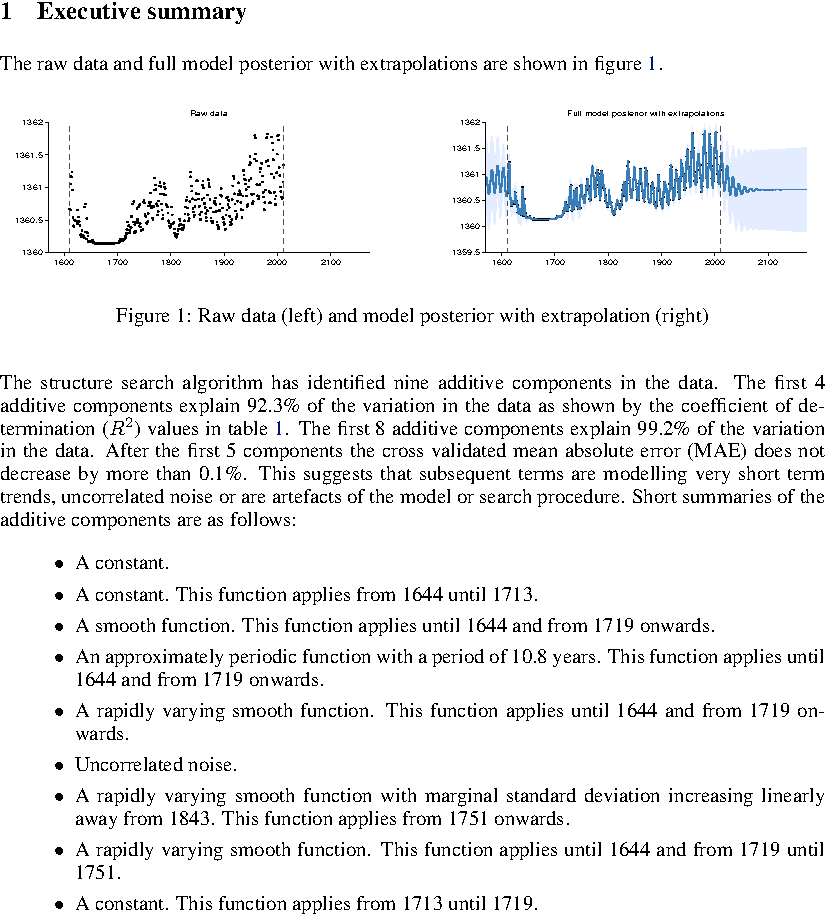
\includegraphics[trim=0cm 11.0cm 9cm 1.7cm, clip, width=0.98\columnwidth]{solarpages/02-solar-seperate-pages-2}}
\caption{
Solar irradiance data.}
\label{fig:solar}
\end{figure}

We show excerpts from the report automatically generated on annual solar irradiation data from 1610 to 2011 (figure~\ref{fig:solar}).
This time series has two pertinent features: a roughly 11-year cycle of solar activity, and a period lasting from 1645 to 1715 with much smaller variance than the rest of the dataset.  This flat region corresponds to the Maunder minimum, a period in which sunspots were extremely rare \citep{lean1995reconstruction}.
The GPSS search procedure and automatic translation clearly identify these two features, as discussed below.

\paragraph{Executive Summary}

The first section of each report gives short summaries about each component in the model, and statistics describing the relative importance of the different components in explaining the data.

\begin{figure}[h]
\centering
\fbox{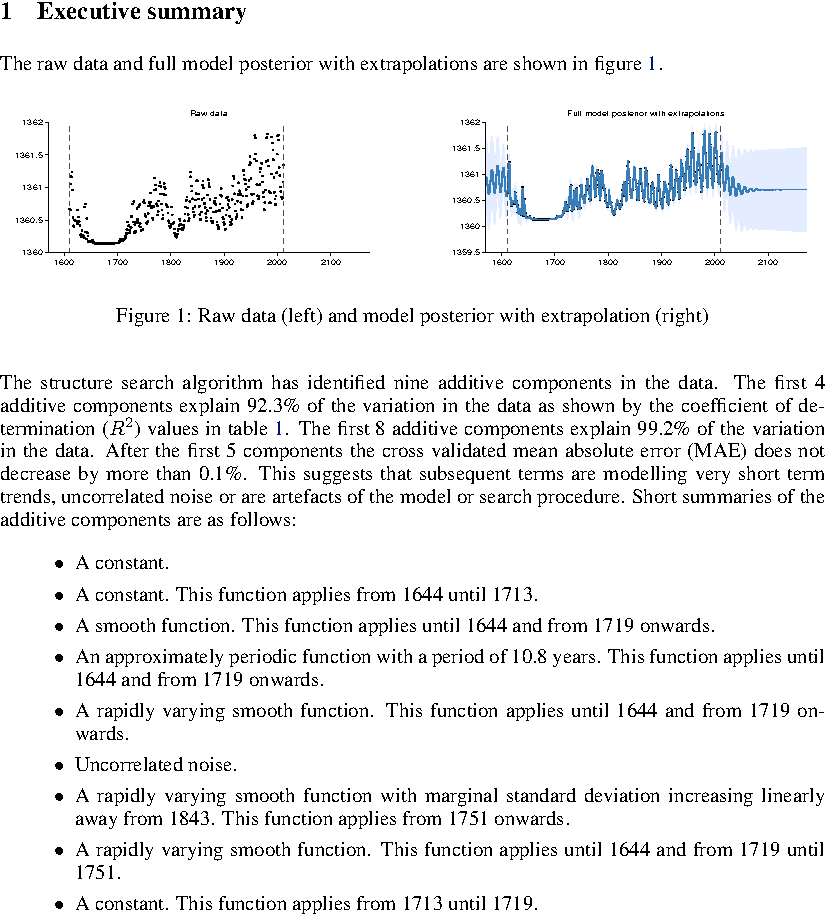
\includegraphics[trim=0cm 3.4cm 0cm 6.3cm, clip, width=0.98\columnwidth]{solarpages/02-solar-seperate-pages-2}}
\caption{
An example of an automatically-generated summary of a dataset.  The dataset is decomposed into diverse types of structures, and each structure is explained in simple terms.}
\label{fig:exec}
\end{figure}

The syntax of the kernels corresponding to the first four components are as follows
\begin{itemize}
  \item $\kC$
  \item $\kCW(\emptyset, \kC)$
  \item $\kCW(\kSE, \emptyset)$
  \item $\kCW(\kSE \times \kPer, \emptyset)$
\end{itemize}
where $\emptyset$ is the zero function.
Figure \ref{fig:exec} shows the automatically-generated summary of the solar dataset.
The short descriptions demonstrate how the kernel is split into univariate enveloping functions (from the change windows) and stationary kernels.
%
%
%The model uses 9 additive components to explain the data, and reports that the first 4 components explain more than 90\% of the variance in the data.
%This might seem incongruous with the observation that there are two main features of the data, but if we examine the first four components, we see that the first component is describing the mean of the dataset, the second is the Maunder minimum, the third describes the long-term trend, and the fourth describes the 11-year periodicity.
Just from the short summaries of the additive components we can see that the model has identified the Maunder minimum (second component) and 11-year solar cycle (fourth component).
%This might seem incongruous with the observation that there are two main features of the data, but if we examine the first four components, we see that the first component is describing the mean of the dataset, the second is the Maunder minimum, the third describes the long-term trend, and the fourth describes the 11-year periodicity.

%\subsubsection{Signal versus Noise}
%
%One design challenge we encountered was seperating the recovered structure into signal and noise.  Originally, the model always included a term corresponding to \iid{} additive Gaussian noise.  However, in practice, the distinction between signal and noise is unclear for two reasons.  First, a component which varies arbitrarily quickly in time can be indistinguishable from noise.  Second, the variance of the noise may change over time (called heteroscedasticity), and this sort of pattern may be considered part of the signal.
%Because of the blurry distinction between signal and noise, we include a table which summarizes the relative contribution of each component in terms of held-out predictive power.%  To do this, we order the components in terms of how much each one improves predictive performance in a 10-fold cross-validation procedure.  The intuition for this metric is that noise-like components do not contribute much to the extrapolation performance of the model, but that signal-like components do.
%
%
%\begin{figure}
%\centering
%\fbox{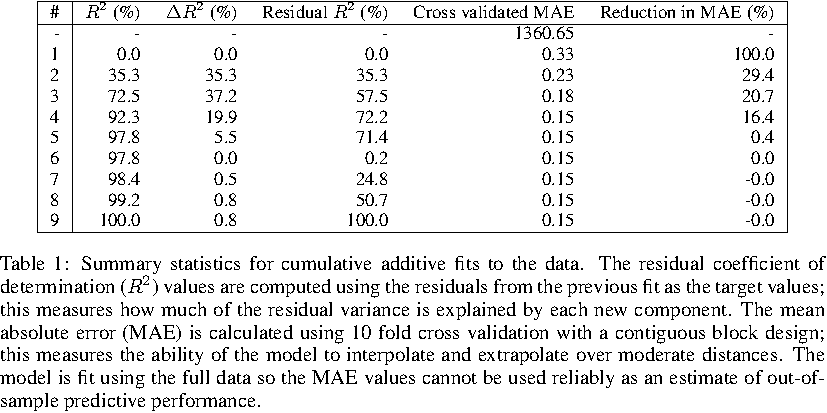
\includegraphics[width=0.98\columnwidth]{solarpages/02-solar-seperate-pages-3}}
%\caption{A table summarizing the relative contribution of the 9 different components of the model in terms of predictive performance.}
%\label{fig:table}
%\end{figure}
%
%Figure \ref{fig:table} show an example of this table on the solar dataset.

%Because the user may be interested in local or noisy components, we report all components to the user.  
%An interactive version of our procedure could allow users to specify which components are of interest, and group the remaining components into a single noise component.

\paragraph{Decomposition plots}

The second section of each report contains a detailed discussion of each component.
%Every component is plotted, and properties of the covariance structure are described.
%Some components are not meaningful when plotted on their own, so we also include plots of the cumulative sum of components.
%\paragraph{Automatic Plotting}
The posterior of the individual component and sum of all components so far is visualised by plots of the posterior mean and variance.
%First, the posterior mean and variance of each component is plotted on its own.
%Second, the posterior mean and variance of all components shown so far is plotted against the data.
%This progression of plots 
%By contrasting each of these plots with plots of earlier components, we can see 
%shows qualitatively how each component contributes to an overall explanation of the data.

%A second paragraph explains the improvement in predictive performance gained by including this component in the model. This is the same informatino as included in the executive summary.

\paragraph{Maunder minimum}

Figure \ref{fig:maunder} shows that GPSS has captured the unusual period of decreased solar activity from about 1645 to 1715 and is able to report this in natural language.

\begin{figure}[ht]
\centering
\fbox{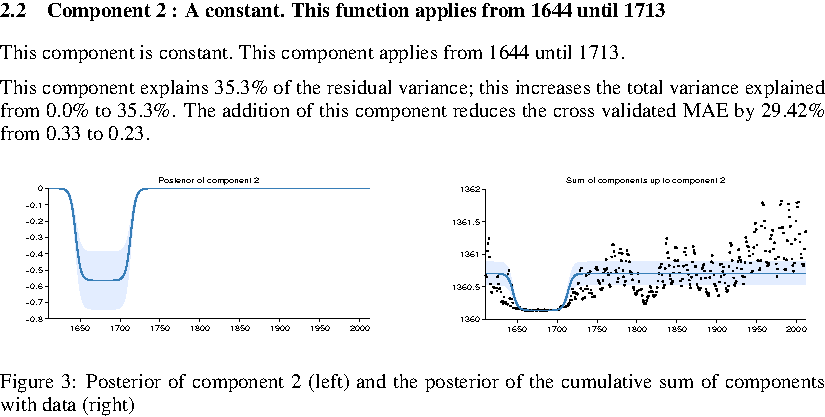
\includegraphics[trim=0cm 0cm 0cm 0.7cm, clip, width=0.98\columnwidth]{solarpages/02-solar-seperate-pages-5}}
\caption{Discovering the Maunder minimum.}
\label{fig:maunder}
\end{figure}

\paragraph{Long term trend}

Having isolated the Maunder minimum, the model captures the long term trend of the rest of the data, shown in figure~\ref{fig:smooth}.

\begin{figure}[h!]
\centering
\fbox{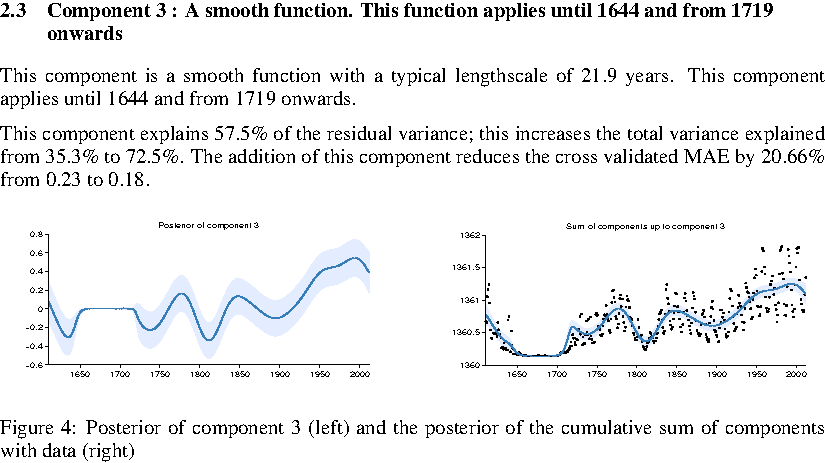
\includegraphics[width=0.98\columnwidth]{solarpages/02-solar-seperate-pages-6}}
\caption{Characterizing the medium-term smoothness of solar activity levels.  By allowing other components to explain the periodicity, noise, and the Maunder minimum, we can isolate the part of the signal best explained by a slowly-varying trend.}
\label{fig:smooth}
\end{figure}

% is a good example of a meaningful component discovered by GPSS, whose meaning would be unclear without an individual plot.  


%In the history of solar activity, the Maunder minimum is a good example of a local change in covariance.  Specifically, 
%The changepoint kernels used by GPSS encode changes in covariance structure.
%For example, from about 1645 to 1715, solar activity decreased.
%, and very few sunspots were observed, a period called the Maunder Minimum \citep{lean1995reconstruction}.
%This feature was captured by the model by multiplying a constant kernel by two changepoint kernels.

\paragraph{Solar cycles}

Figure \ref{fig:periodic} shows that GPSS has isolated the approximately 11 year solar cycle.
By examining the parameters of the kernels comprising this component the description identifies that the shape of the periodicity is near sinusoidal \NA{(it does in the latest version)} and also quantifies how quickly the exact shape of the sinusoid changes.

%with a pair of changepoint kernels.%shows exactly which sort of structure was recovered by this component.
%
%\begin{figure}[h!]
%\centering
%\fbox{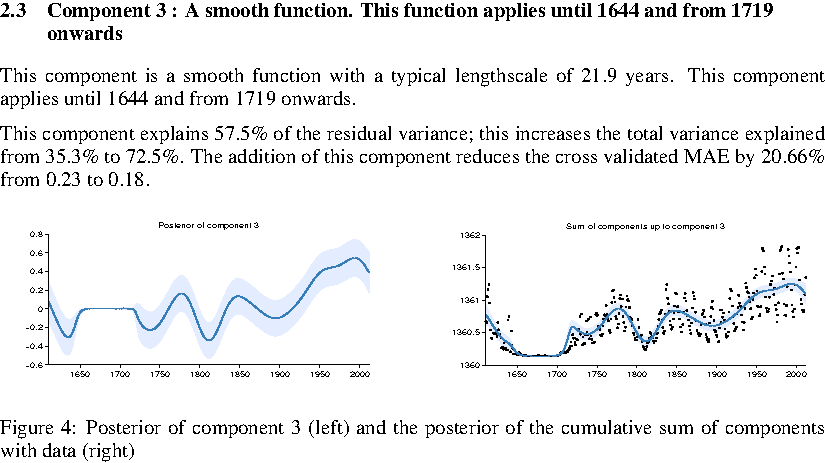
\includegraphics[width=0.98\columnwidth]{solarpages/02-solar-seperate-pages-6}}
%\caption{Characterizing the medium-term smoothness of solar activity levels.  By allowing other components to explain the periodicity, noise, and the Maunder minimum, we can isolate the part of the signal best explained by a slowly-varying trend.}
%\label{fig:smooth}
%\end{figure}

%\paragraph{Isolating the smoothly-varying component} Examining the dataset by eye, overall solar activity seems to change slowly over decades.  However, this intuition seems difficult to formalize.  Linear or quadratic regression is clearly inappropriate, and methods based on local smoothing would need to control for the periodic component.  Luckily, the GPSS procedure does exactly this, allowing us to isolate the slowly-varying component of the data, without having to forecast either the Maunder minimum or the periodic variation.  Figure \ref{fig:smooth} shows the automatically-generated summary of this component.

\begin{figure}[ht]
\centering
\fbox{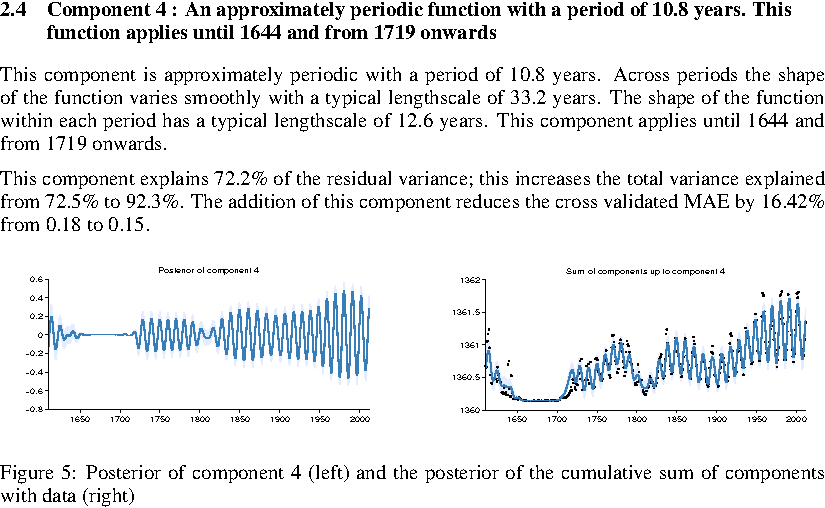
\includegraphics[trim=0cm 0cm 0cm 1.0cm, clip, width=0.98\columnwidth]{solarpages/02-solar-seperate-pages-7}}
\caption{Isolating the periodic component of the dataset.  By isolating this aspect of the statistical structure, we can easily observe additional features, such as the shape of the peaks and troughs, or the fact that the amplitude changes over time.}
\label{fig:periodic}
\end{figure}

%Figure \ref{fig:periodic} shows that GPSS has identified the approximately 11 year solar cycle.
%By isolating this component in separate plots it is easy to see the exact nature of the solar cycle \eg how the amplitude of this periodic component varies over time.
%This demonstrates one benefit of isolating individual components: we can now see, by eye, extra structure that was not explicitly captured by the model.  Specifically, we can see that the amplitude of the periodic component varies over time.

%and by comparing with figure \ref{fig:smooth}, we can see that it varies roughly in proportion to the overall magnitude of the signal.
%  This pattern suggests that some sort of log-transform might be appropriate for this dataset, or that the model should be extended in some way to capture this structure.

%\paragraph{Extrapolation plots}
%
%The third section of each report shows extrapolations into the future, as well as posterior samples from each individual component of the model.  These samples help to characterize the uncertainty expressed by the model, and the extent to which different components contribute to predicting the future behavior of a time series.
%%
%The predictive mean and variance of the signals shown in the summary plots are useful, but do not capture the joint correlation structure in the posterior.  Showing posterior samples is a simple and universal way to illustrate joint statistical structure.
%%
%\begin{figure}[ht]
%\centering
%\fbox{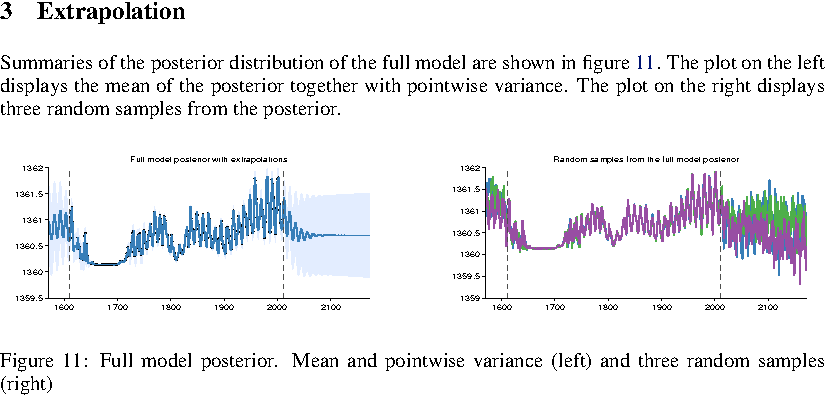
\includegraphics[trim=0cm 0cm 0cm 2.8cm, clip, width=0.98\columnwidth]{solarpages/02-solar-seperate-pages-13}}
%\caption{Sampling from the posterior.  These samples help show not just the predictive mean and variance, but also the predictive covariance structure.  Note, for example, that the predictive mean (left) does not exhibit periodicity, but the samples (right) do.}
%\label{fig:extrap-full}
%\end{figure}
%%
%For example,
%%  shows the predictive mean and variance given the entire model. 
%it is not clear from the left-hand plot in figure \ref{fig:extrap-full} whether or not the periodicity of the dataset is expected to continue into the future.  However, from the samples on the right-hand size, we can see that this is indeed the case.  

%\begin{figure}[h!]
%\centering
%\fbox{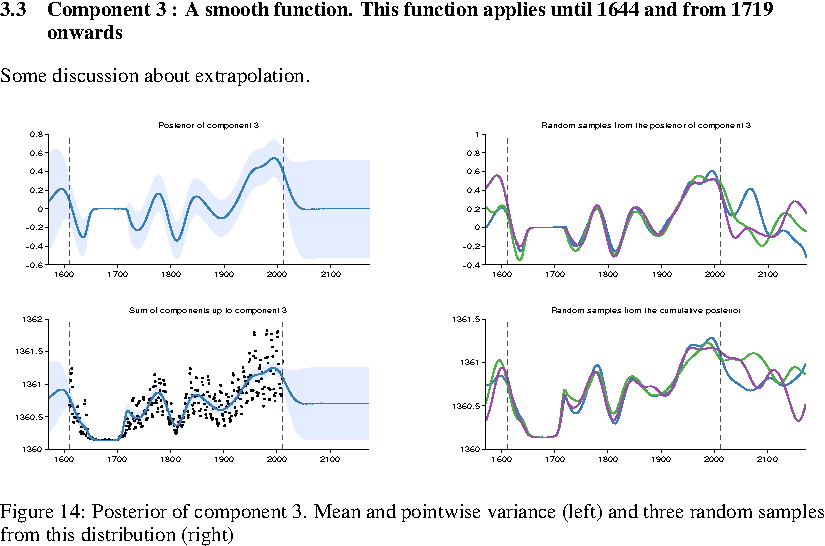
\includegraphics[width=0.98\columnwidth]{solarpages/02-solar-seperate-pages-16}}
%\caption{Extrapolating a single component of the model.  Because our model class allows us to isolate individual components, we can show the extent to which the model expects different trends to continue.  We also observe that the posterior samples are quite different from the posterior mean, away from the data.}
%\label{fig:extrap-smooth}
%\end{figure}

%\paragraph{Extrapolating individual components}
%We can also examine the model's expectations about the future behavior of individual components through sampling.  Further plots in the extrapolation section show posterior samples for each individual additive component. %For example, in figure \ref{fig:extrap-smooth}, we are shown samples of the predictive distribution of the smooth component of variation.  This plot indicates that the model considers a wide range of future average intensities to be plausible, but that it always expects those average intensities to vary smoothly.

%\section{Related Work}

%There exists a vast literature on both model visualization and model checking.


%\paragraph{Structure learning in Bayesian networks}
%Similar idea of discovering semantics via model search.
%Semantics are more vague though \ie a probability table is not an entirely concise summary

%\paragraph{Linear model}
%These discover highly interpretable semantics but are limited in expressivity

%\paragraph{Nonparametric additive models}
%Highly flexible but semantics are vague \ie can only talk about smooth functions

%\paragraph{Equation learning}
%Very flexible but semantics of equations do not map onto human understanding \eg saw tooth vs Fourier decomposition of a saw tooth - which is more human understandable?
%How would you explain a sensor error with Eureqa style equations.

%\paragraph{Deep learning}
%Again very flexible but the semantics are not usually human interpretable.
%How can we understand the output of complex representation learning algorithms without human intervention (\eg recognising that your deep net has become a cat classifier).

%\paragraph{Kernel search}
%Can use the precise semantics of linear models or the vague semantics of nonparametric additive models and other components along this spectrum.
%Flexible modelling with components that a human might use to describe what is going on.

\subsection{Describing heteroscedasticity}
\label{sec:airline}

\begin{figure}[h]
\centering
\fbox{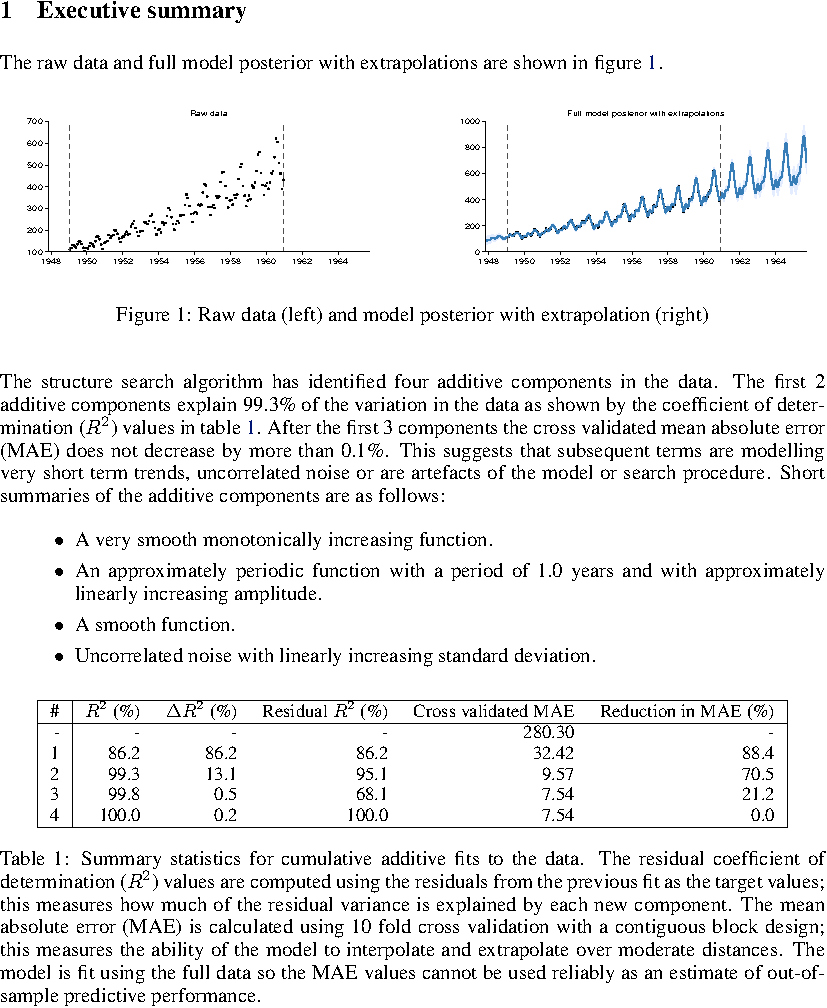
\includegraphics[trim=0cm 12.5cm 9cm 1.7cm, clip, width=0.98\columnwidth]{airlinepages/01-airline-separate-pages-2}}
\caption{
International airline passenger data.}
\label{fig:airline}
\end{figure}

We also analysed international airline passenger data (figure~\ref{fig:airline}).
The model constructed by GPSS has four components with the following syntax and descriptions given in figure~\ref{fig:exec-airline}.
\begin{itemize}
  \item $\kSE$
  \item $\kSE \times \kPer \times \kLin$
  \item $\kSE$
  \item $\kWN \times \kLin$
\end{itemize}

\begin{figure}[h]
\centering
\fbox{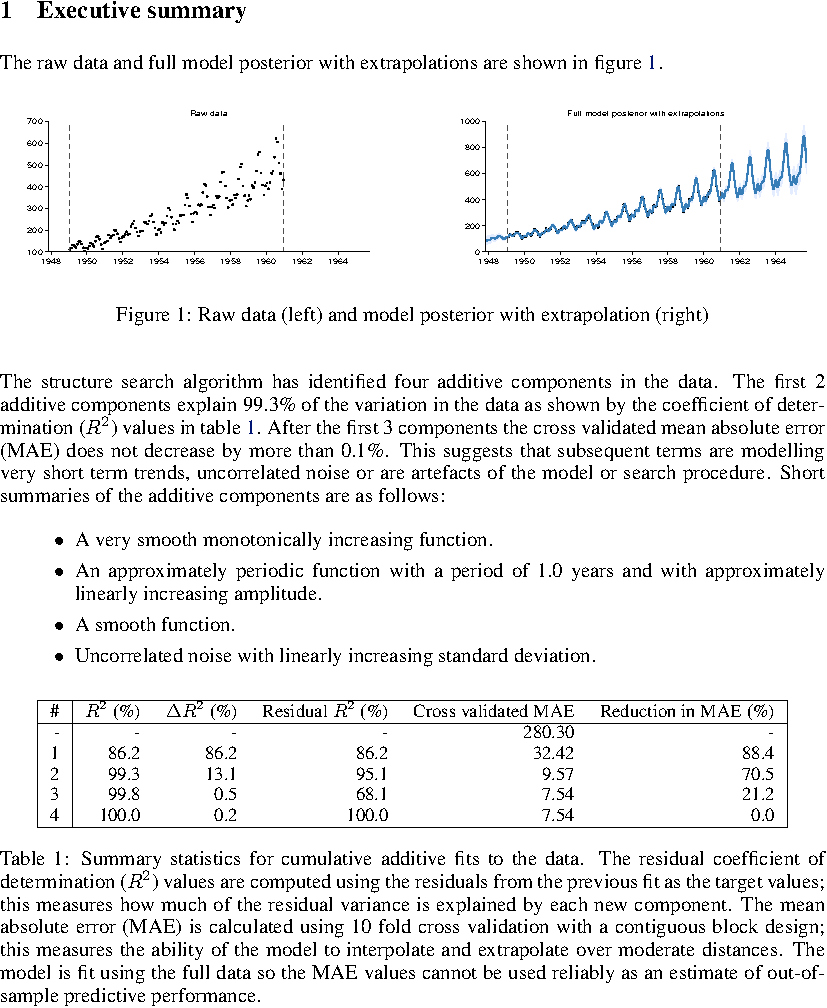
\includegraphics[trim=0cm 3cm 0cm 6cm, clip, width=0.98\columnwidth]{airlinepages/01-airline-separate-pages-2}}
\caption{
Short descriptions and summary statistics for the four components of the airline model.}
\label{fig:exec-airline}
\end{figure}

\paragraph{Monotonic trend}

No kernel in the current language can express a prior over monotonic functions.
However, it is simple to check the posterior for monotonicity and remark upon it when appropriate (figure~\ref{fig:monotonic}).

\begin{figure}[h]
\centering
\fbox{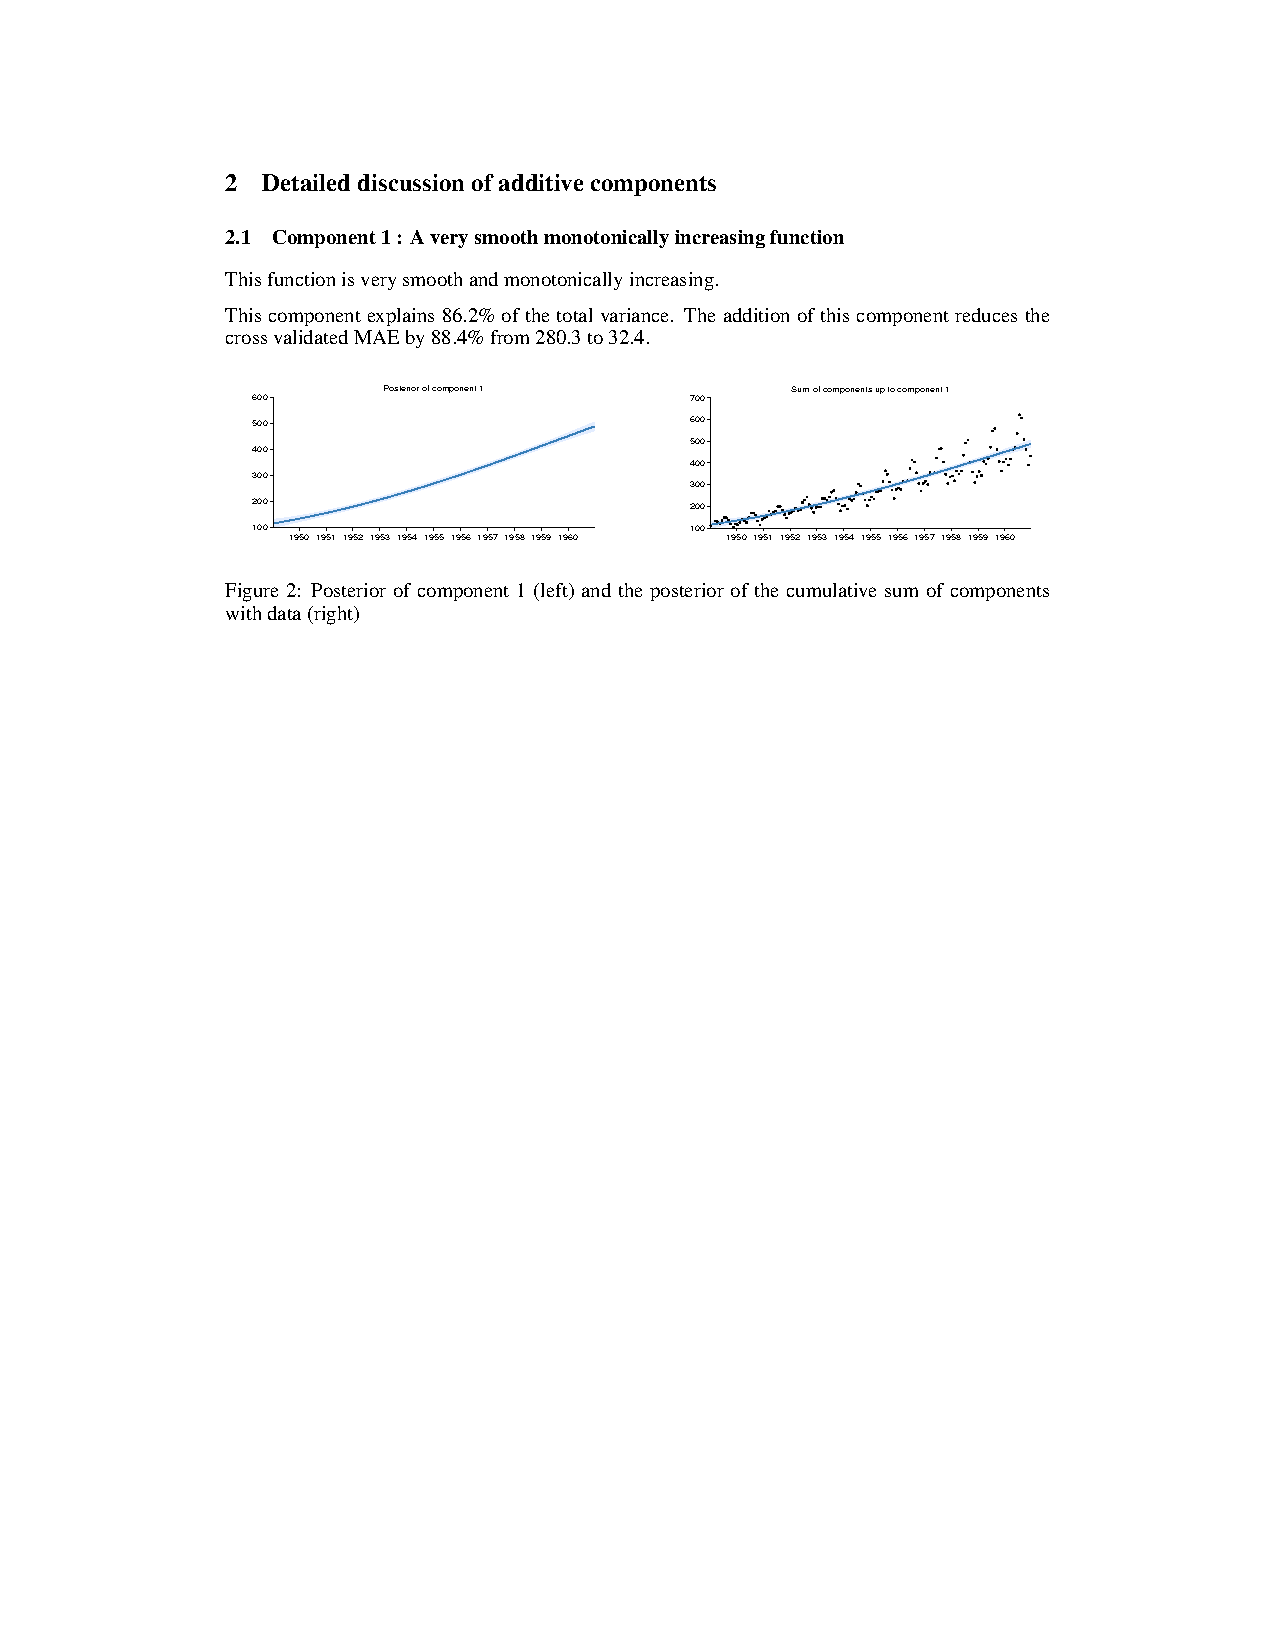
\includegraphics[trim=0cm 0cm 0cm 0cm, clip, width=0.98\columnwidth]{airlinepages/01-airline-separate-pages-3}}
\caption{Describing monotonicity of the posterior}
\label{fig:monotonic}
\end{figure}

\paragraph{Annual periodicity with linearly growing amplitude}

The second component (figure~\ref{fig:lin_periodic}) is correctly identified as approximately ($\kSE$) periodic ($\kPer$) with linearly growing amplitude ($\kLin$).

\begin{figure}[h]
\centering
\fbox{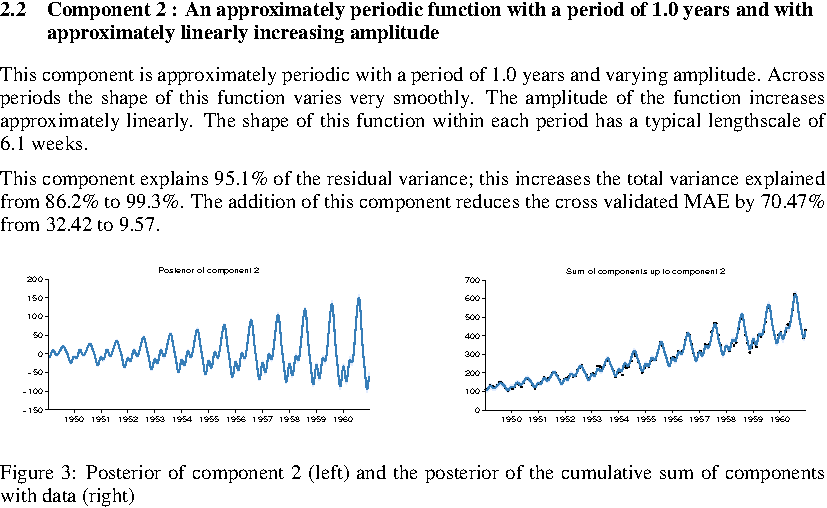
\includegraphics[trim=0cm 0cm 0cm 0cm, clip, width=0.98\columnwidth]{airlinepages/01-airline-separate-pages-4}}
\caption{Capturing non-stationary periodicity in the airline data}
\label{fig:lin_periodic}
\end{figure}

%\begin{figure}[h]
%\centering
%\fbox{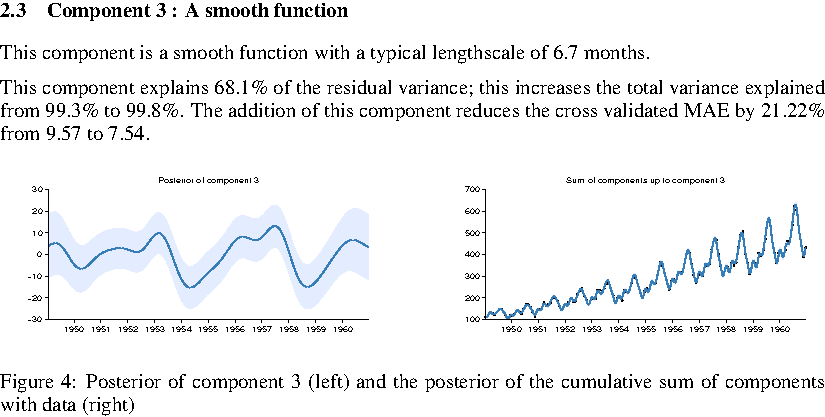
\includegraphics[trim=0cm 17cm 0cm 3.5cm, clip, width=0.98\columnwidth]{airlinepages/01-airline-separate-pages-5}}
%\caption{
%A caption.}
%\label{fig:exec}
%\end{figure}

\paragraph{Linear heteroscedasticity}

By multiplying a white noise kernel by a linear kernel the model is able to express heteroscedasticity (figure~\ref{fig:heteroscedastic}).

\begin{figure}[h]
\centering
\fbox{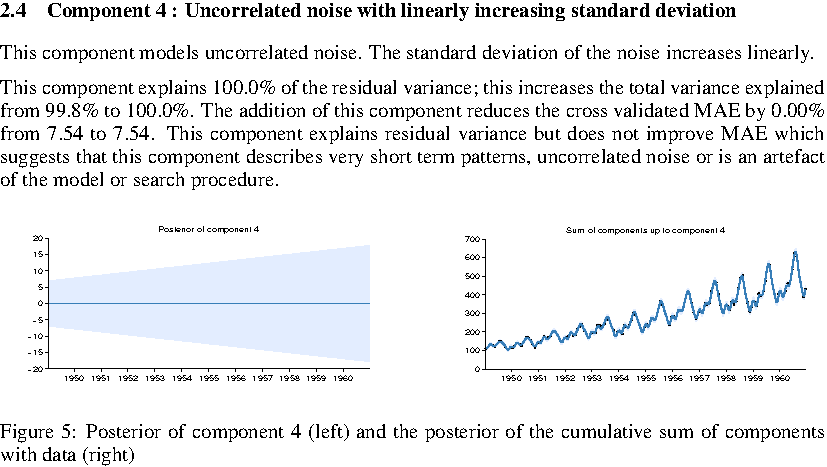
\includegraphics[trim=0cm 0cm 0cm 0cm, clip, width=0.98\columnwidth]{airlinepages/01-airline-separate-pages-6}}
\caption{Modelling heteroscedasticity}
\label{fig:heteroscedastic}
\end{figure}

\subsection{Comparison to equation learning}

The vast majority of machine learning algorithm research focuses on numerical performance, with claims of interpretability generated post-hoc.
Another method which attempts to automate the process of interpretation is that of equation learning (cite), where a regression function is described via a parametric equation.

We include learned equations for these two data sets for completeness; however, it is very unlikely that these data sets can be explained parsimoniously with a parametric function.

The learned equation\fTBD{give details of procedure} for the solar data is
\begin{equation}
\textrm{Irradiance} = 1361 + \alpha\sin(\beta + \gamma t)\sin(\delta + \epsilon t^2 - \zeta t)
\end{equation}
where $t$ is time (the input to the regression) and we have replaced most constants with symbols for brevity.
This equation captures the constant offset of the data and models the long term trends with a product of sinusoids but fails to capture the solar cycle or the Maunder-minimum.

The learned equation for the airline data is
\begin{equation}
\textrm{Passengers} = \alpha t + \beta\cos(\gamma - \delta t)\textrm{logistic}(\epsilon t - \zeta) - \eta
\end{equation}
which captures the approximately linear trend, and the periodic component with approximately linearly increasing amplitude.
However, the periodicity is heavily approximated with only a single sinusoid.

\section{Numerical evaluation}
\label{sec:numerical}

To complement our demonstration of the interpretability of our method, we conducted numerical experiments testing the ability of various model building algorithms to interpolate and extrapolate time-series.
GPSS outperforms the other methods on average (\eg as measured by quantiles of performance metrics) but the differences between the top performing methods are small.

\paragraph{Data sets}

In addition to the three time series analysed in \cite{DuvLloGroetal13} we evaluate the performance of GPSS and 5 other algorithms on 10 additional time series from (cite time series data library); plots are given in the appendix.

\paragraph{Algorithms}

We compare the structure search algorithm to equation learning \cite{Schmidt2009b} and four other regression algorithms; multiple kernel learning (cite), change point modelling (cite) / multi resolution Gaussian processes (cite), spectral kernels (cite) and trend-cyclical-irregular (cite).
These four algorithms can be expressed as restrictions of our modelling language (see table~\ref{table:motifs}).
\NA{Give more details of inference procedures}

We restrict to regression algorithms for comparability; this excludes models which regress on previous values of times series (\eg cite ARIMA or similar).
Producing model construction algorithms for this class of time-series model would be an interesting area for future research.

\paragraph{Interpolation}

To test the ability of the methods to interpolate, we randomly divided each data set into equal amounts of training data and testing data.
We trained each algorithm on the training half of the data, produced predictions for the remaining half and then computed the root mean squared error (RMSE).
The values of the RMSEs are then standardised by dividing by the smallest RMSE for each data set \ie the best performance on each data set will have a value of 1.

Figure~\ref{fig:box_interp} shows the standardised RMSEs for the different algorithms (raw data and bow plots).
The box plots demonstrate that all quartiles of the distribution of standardised RMSEs are lower for GPSS.
However, the medians and largest outliers of GPSS, SP and TCI are all quite similar in value so we should conclude that all methods are similarly effective at interpolation.

\begin{figure}[h]
\centering
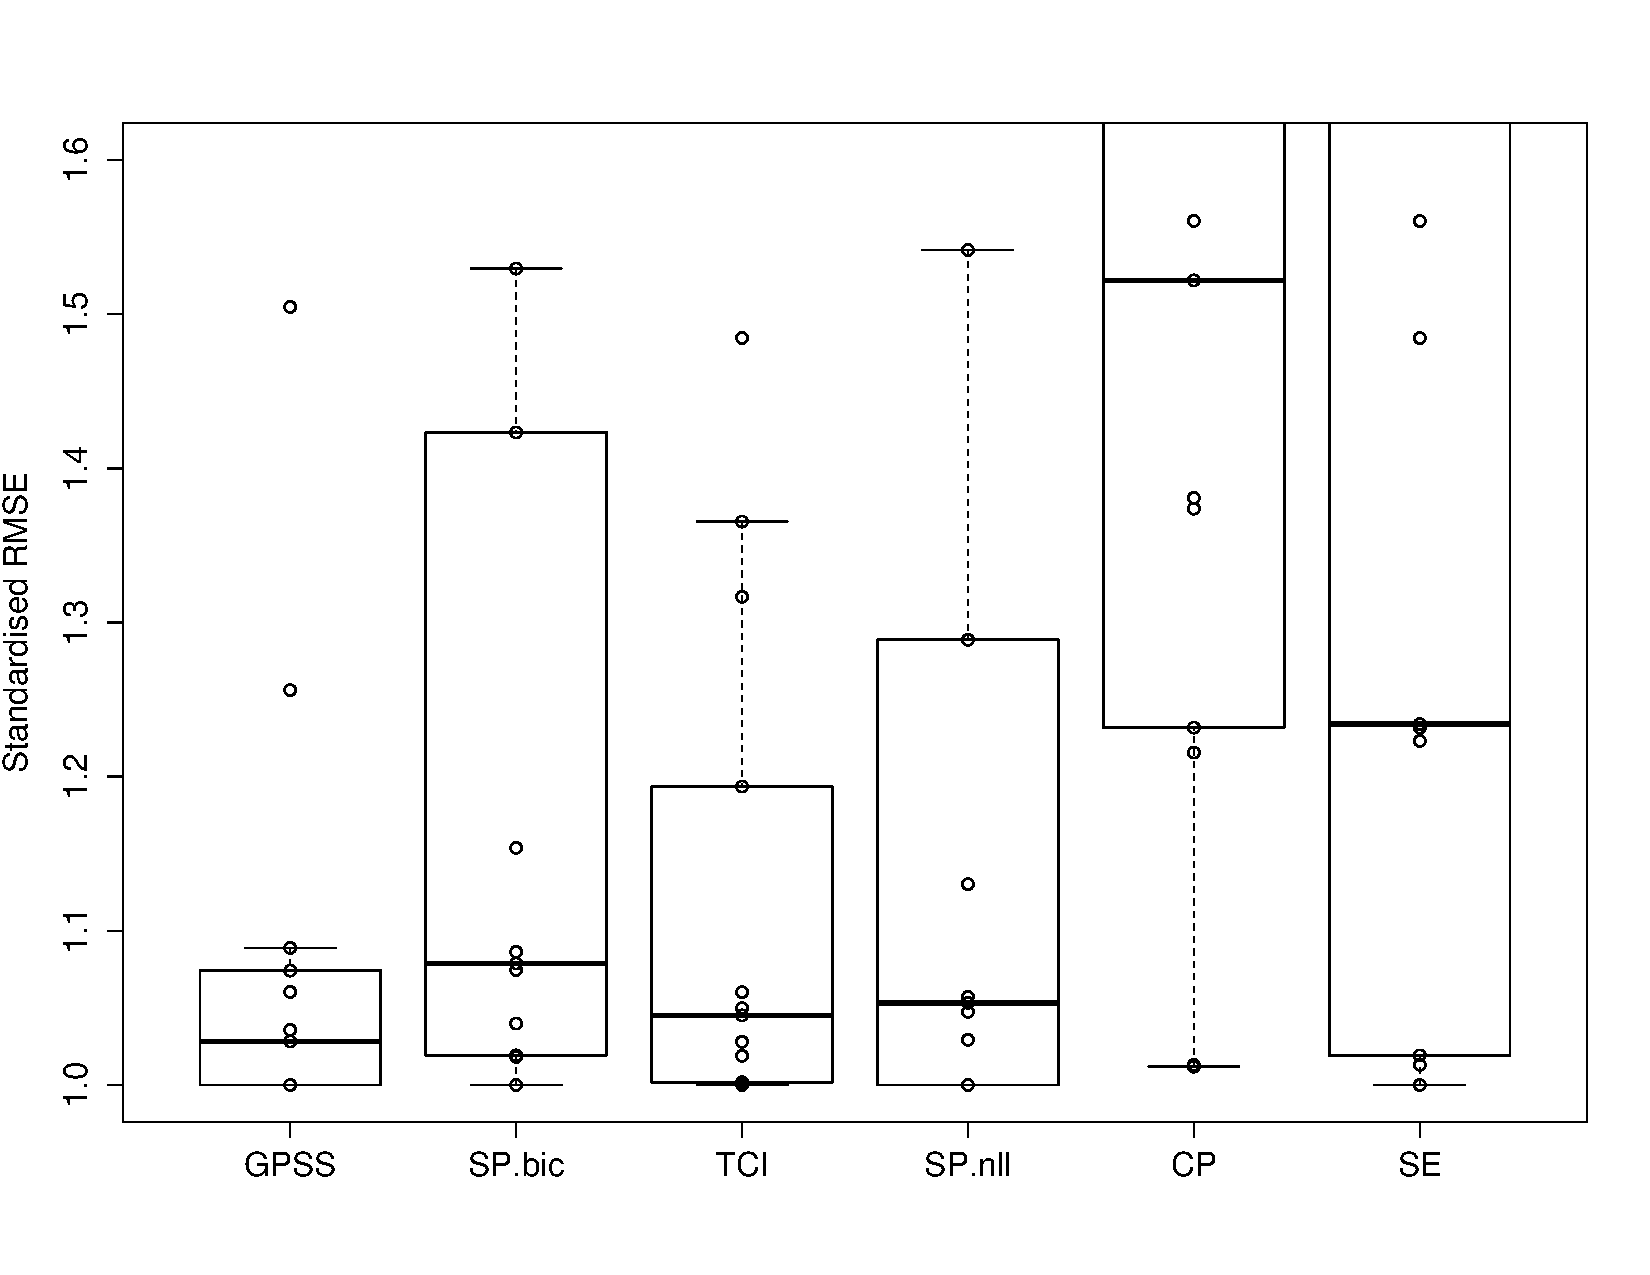
\includegraphics[width=\columnwidth]{figures/box_interp}
\caption{
Raw data, and box plot of standardised interpolation RMSE (best performance = 1).
}
\label{fig:box_interp}
\end{figure}

CP performs worse than all other methods despite including SE as a special case in its grammar.
The introduction of CP allows for more interpretable models, but it introduces parametric forms into the regression models (\ie the sigmoids expressing the changepoints).
This results in worse interpolations at the locations of the change points, suggesting that a more robust modelling language would require a more flexible class of changepoint shapes or improved inference (\eg fully Bayesian inference over the location and shape of the changepoint like (cite something)).

\paragraph{Extrapolation}

To test extrapolation we trained all algorithms on the first 90\% of the data, and attempted to predict the remaining 10\%.
Figure~\ref{fig:box_log_extrap} shows the standardised log RMSEs across algorithms.
GPSS again has lower quantiles than all other methods but the differences between GPSS, SP and TCI are small compared to the variance of the results so we cannot conclude that any method is a clear winner.

\begin{figure}[h]
\centering
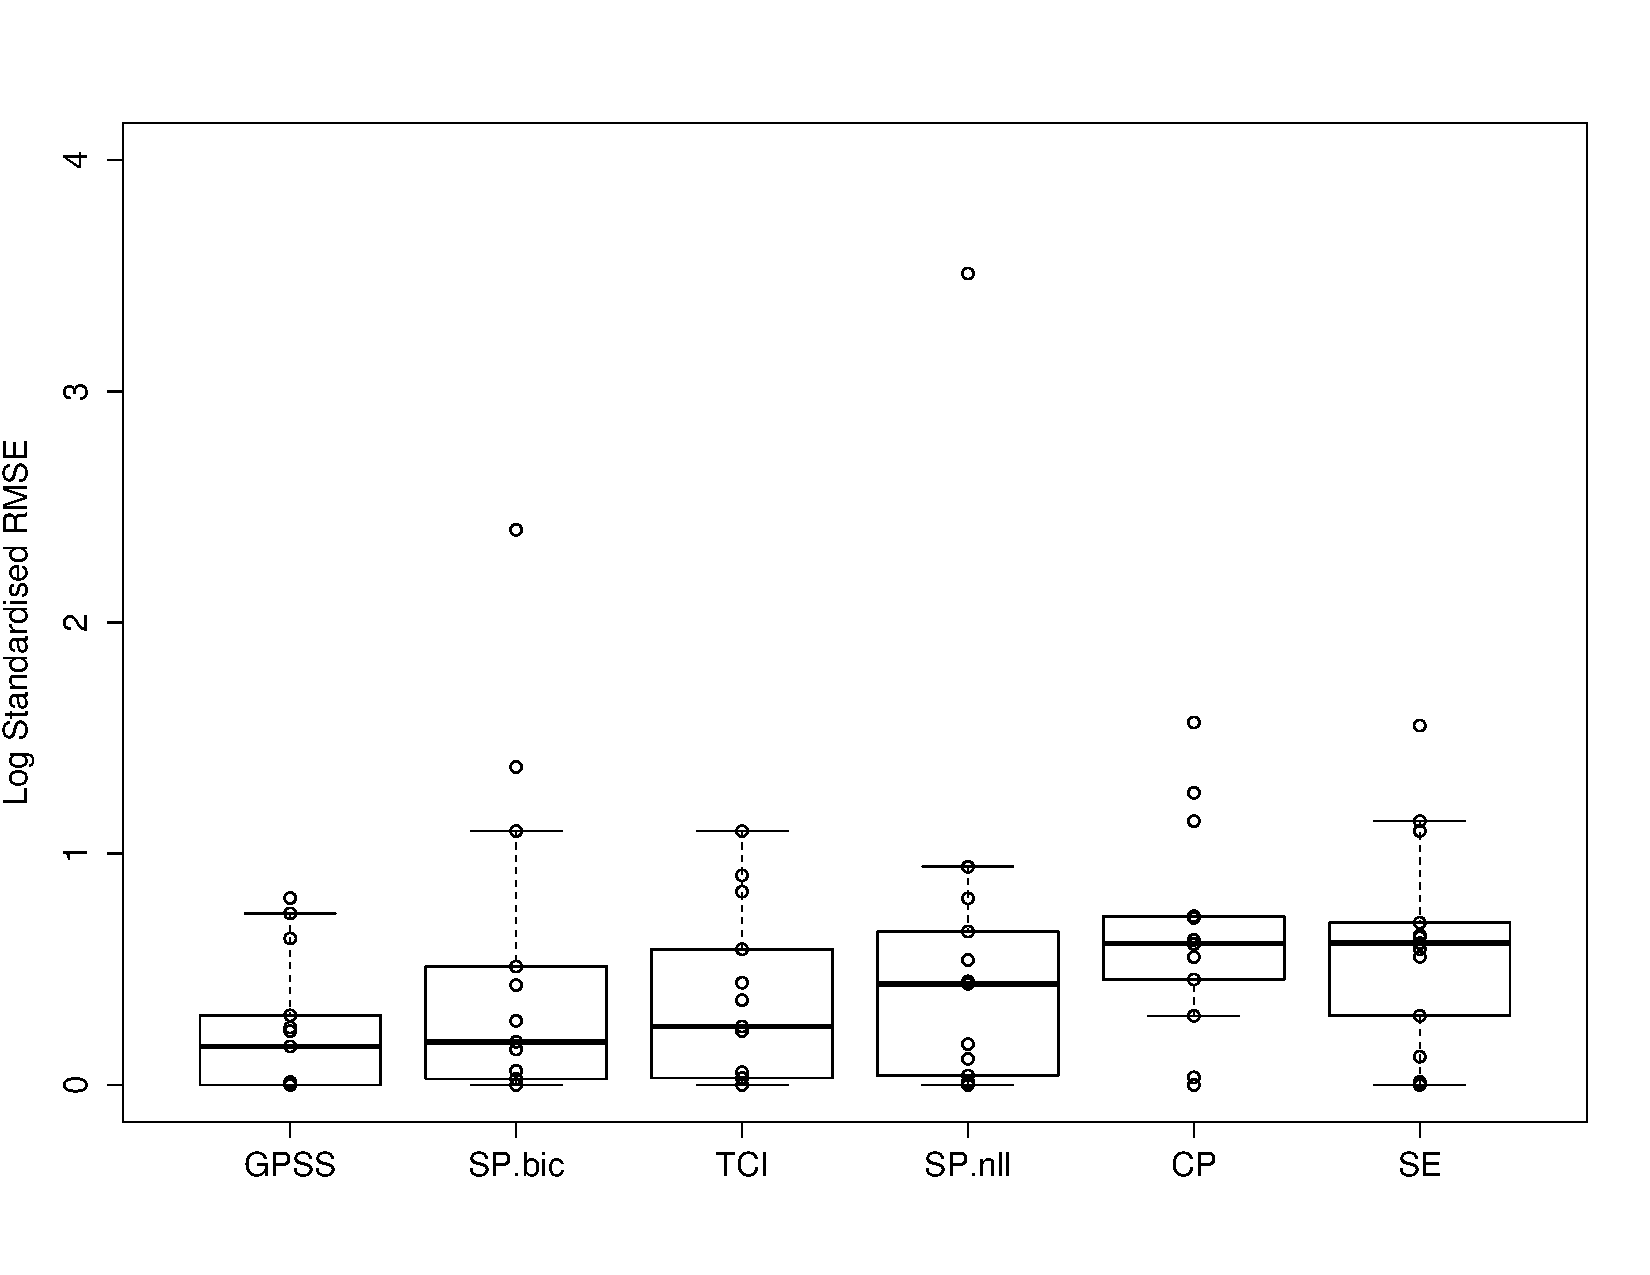
\includegraphics[width=\columnwidth]{figures/box_log_extrap}
\caption{
Raw data, and box plot of log standardised extrapolation RMSE (best performance = 0).
Ordered by median.
}
\label{fig:box_log_extrap}
\end{figure}

%\begin{figure}[h]
%\centering
%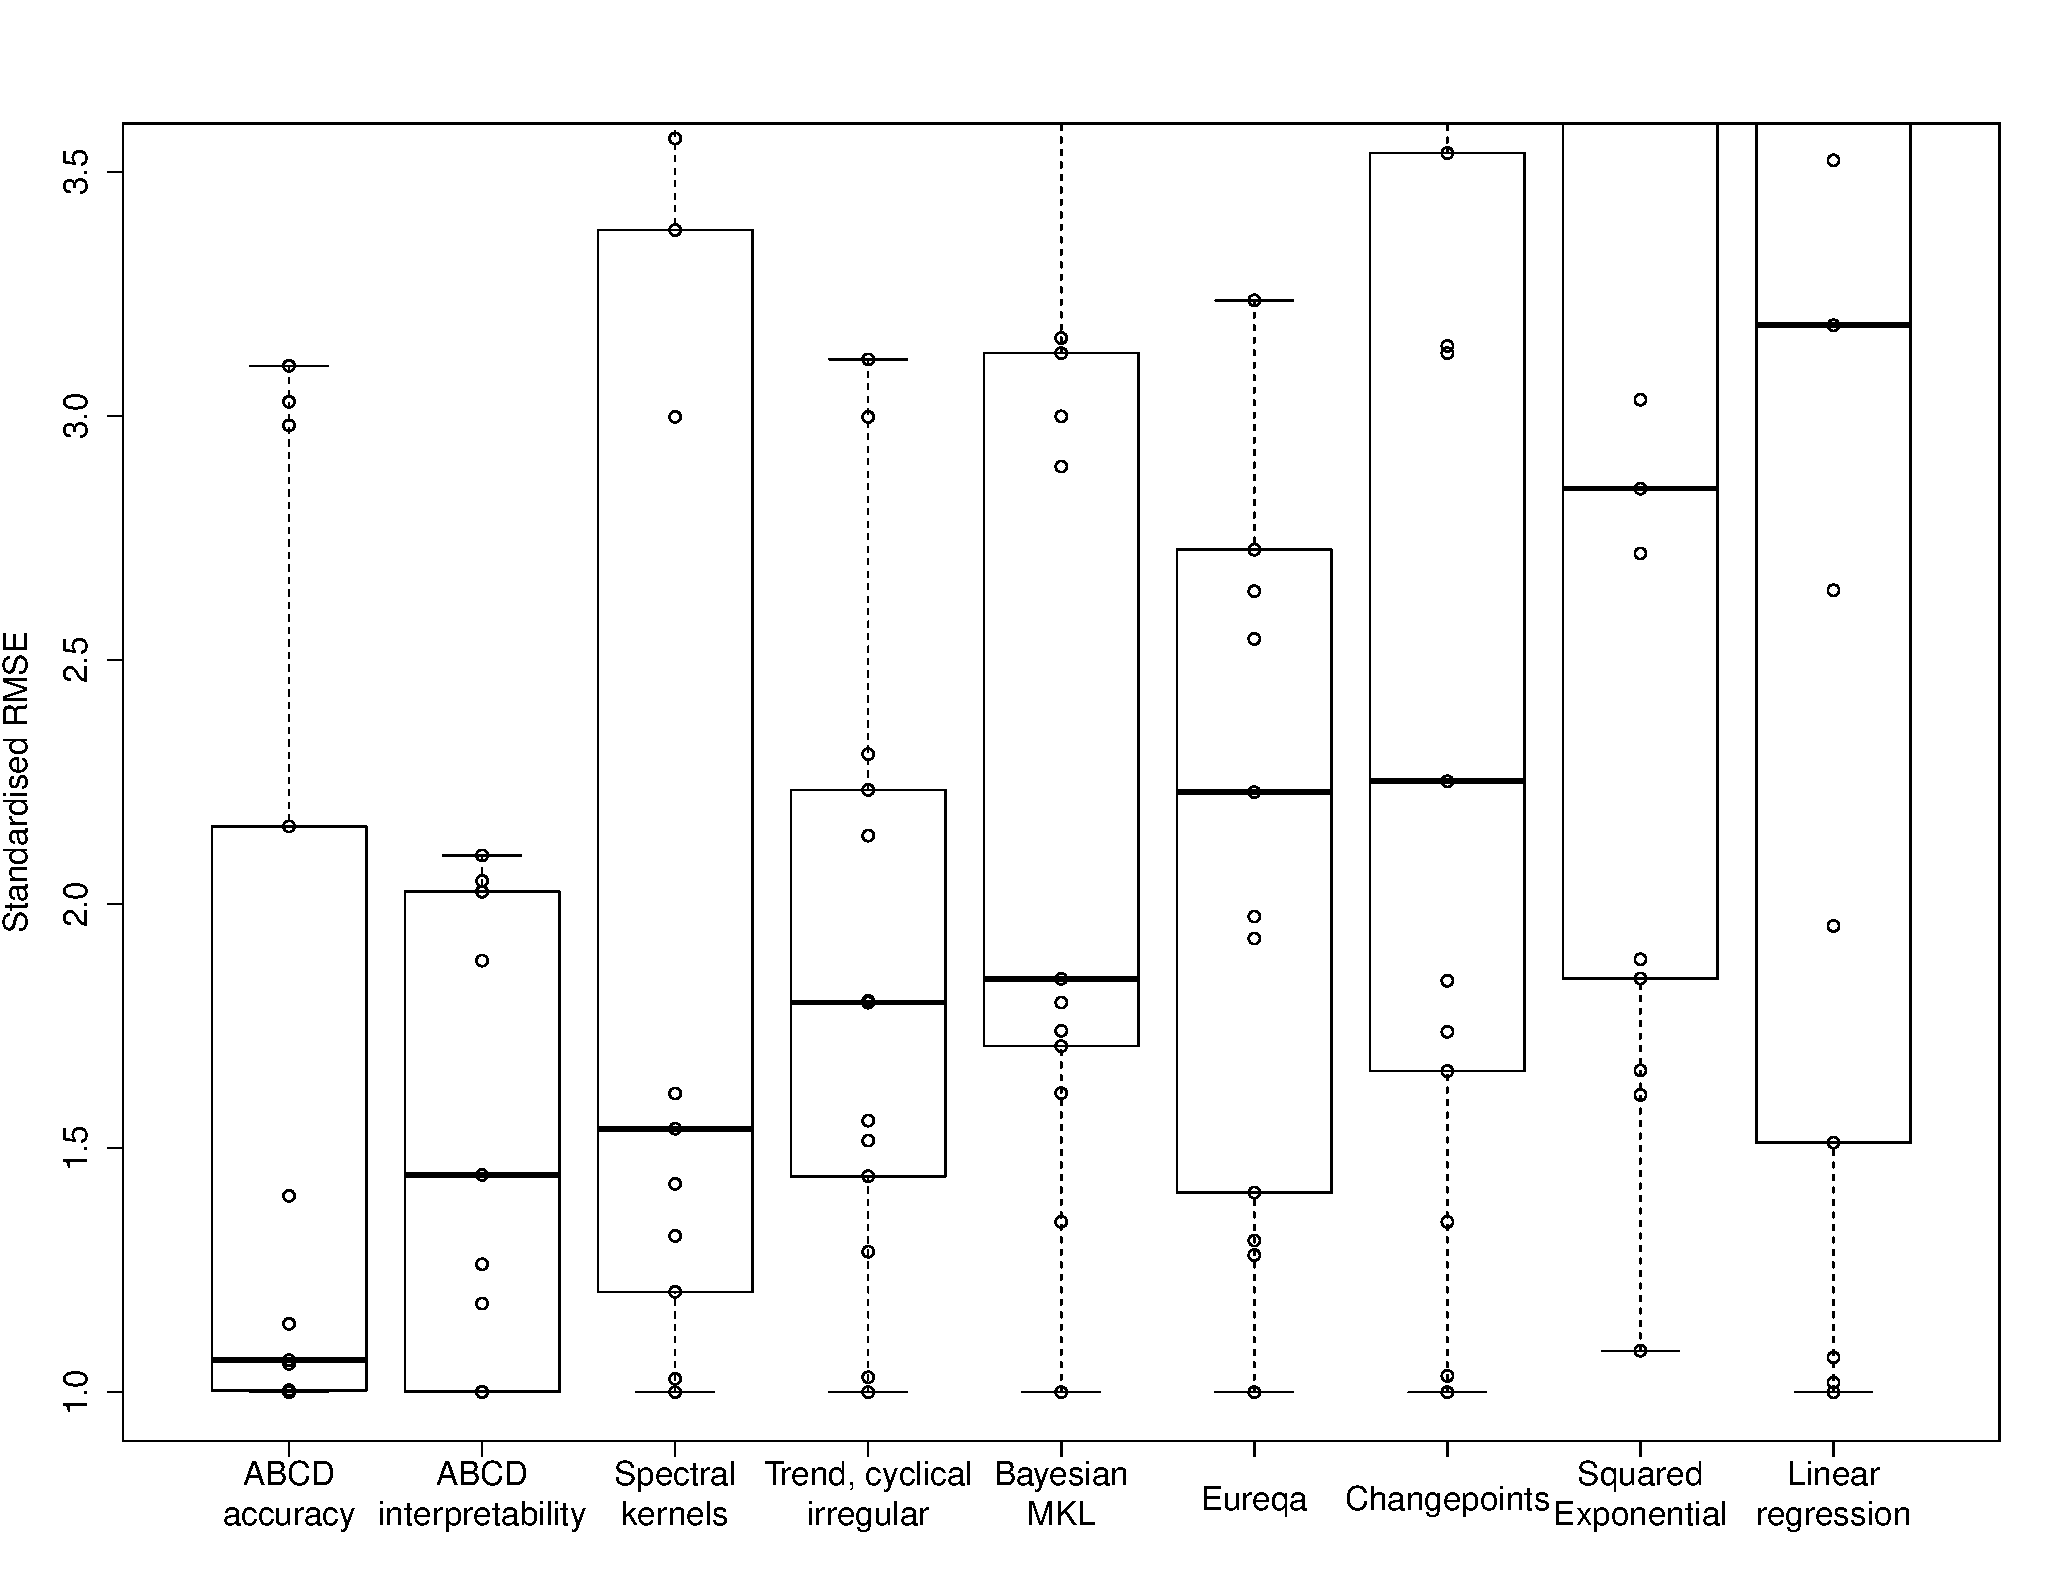
\includegraphics[width=\columnwidth]{figures/box_extrap}
%\caption{
%Raw data, and box plot of standardised extrapolation RMSE (best performance = 1).
%Outlier is the two spectral kernel methods (SP) are not shown.
%}
%\label{fig:box_extrap}
%\end{figure}

SP suffered from very large outliers on a dataset with a large and sharp discontinuity (see the call centre data in the supplementary material) which violates its assumptions of stationarity.
In contrast, GPSS was the best performing algorithm on this dataset, correctly modelling the dataset as locally stationary using change points.

Somewhat surprisingly, TCI performs well despite its restrictive modelling assumptions (smooth functions and exact periodicity).
Further inspection of the extrapolation has revealed that while TCI cannot model non-stationarity, its extrapolations of approximately periodic components can be quite effective.
While GPSS and SP will quickly become uncertain about a roughly periodic component, TCI will predict the average which is often more effective.
This suggests that models composed of kernels of the form $(\kSE + \kC) \times \kPer$ will be effective for extrapolating approximately periodic components.

\section{Discussion}

\TBD{Have another go at this}

The contributions of this paper are two-fold
\begin{itemize}
  \item An expanded model construction algorithm for regression with superior interpolation and extrapolation performance compared to other model construction motifs
  \item The automatic translation of any model expressible in our language of kernels into natural-language
\end{itemize}
The first is a traditional contribution to machine learning or statistical methodology.
The second is clear to any researcher familiar with Gaussian processes or related techniques.
However, in sum this manuscript is a contribution to artificial intelligence, automating a part of the process of statistical analysis that is currently performed by humans.

\paragraph{Disconnected notes}

\NA{
Please feel free to note down anything that seems sensible to discuss here - I am yet to think of a definitive conclusion.
}

\NA{
We should demand the same transparency of statistical models as we do a junior employee - although continuing the analogy we sometimes do not expect transparency from a genius (deep neural nets? - j/k).
}

\NA{
If we can explain something in plain language then we should.
}

\NA{
What are the correct metrics?
A good description should reflect a statistical model that can predict well.
Interpolation and extrapolation are one measure of prediction.
Another measure could be scientific discovery - this feels like the ultimate test.
}

\paragraph{Source Code}
Source code to perform all experiments is available on github.\footnote{
\href{http://www.github.com/jamesrobertlloyd/gpss-research}
{\texttt{github.com/jamesrobertlloyd/gpss-research}}}
%All \gp{} hyperparameter tuning was performed by automated calls to the GPML toolbox\footnote{Available at 
%\href{http://www.gaussianprocess.org/gpml/code/}
%{\texttt{www.gaussianprocess.org/gpml/code/}}
%}

%\section{Discussion}

%\begin{quotation}
%``The availability of 'user-friendly' statistical software has caused authors to become increasingly careless about the logic of interpreting their results, and to rely uncritically on computer output, often using the 'default option' when something a little different (usually, but not always, a little more complicated) is correct, or at least more appropriate.''
% In trying to practice this art, the Bayesian has the advantage because his formal apparatus already developed gives him a clearer picture of what to expect, and therefore a sharper perception for recognizing the unexpected.

%\defcitealias{dyke1997avoid}{G. Dyke, 1997}
%\hspace*{\fill}\citet{Jaynes85highlyinformative}
%\hspace*{\fill}\citetalias{dyke1997avoid}
%\end{quotation}

%In this paper, we exhibited the output of a method for automatically constructing and summarizing a compositional Gaussian process regression model in natural language.
%These summaries can enable human experts and non-experts to understand the implications of a model, check its plausibility, and notice structure not yet captured by the model.

\bibliography{gpss}
\bibliographystyle{format/icml2014}

\end{document} 
